\documentclass[a4paper]{article}\usepackage[]{graphicx}\usepackage[]{color}
%% maxwidth is the original width if it is less than linewidth
%% otherwise use linewidth (to make sure the graphics do not exceed the margin)
\makeatletter
\def\maxwidth{ %
  \ifdim\Gin@nat@width>\linewidth
    \linewidth
  \else
    \Gin@nat@width
  \fi
}
\makeatother

\definecolor{fgcolor}{rgb}{0.345, 0.345, 0.345}
\newcommand{\hlnum}[1]{\textcolor[rgb]{0.686,0.059,0.569}{#1}}%
\newcommand{\hlstr}[1]{\textcolor[rgb]{0.192,0.494,0.8}{#1}}%
\newcommand{\hlcom}[1]{\textcolor[rgb]{0.678,0.584,0.686}{\textit{#1}}}%
\newcommand{\hlopt}[1]{\textcolor[rgb]{0,0,0}{#1}}%
\newcommand{\hlstd}[1]{\textcolor[rgb]{0.345,0.345,0.345}{#1}}%
\newcommand{\hlkwa}[1]{\textcolor[rgb]{0.161,0.373,0.58}{\textbf{#1}}}%
\newcommand{\hlkwb}[1]{\textcolor[rgb]{0.69,0.353,0.396}{#1}}%
\newcommand{\hlkwc}[1]{\textcolor[rgb]{0.333,0.667,0.333}{#1}}%
\newcommand{\hlkwd}[1]{\textcolor[rgb]{0.737,0.353,0.396}{\textbf{#1}}}%

\usepackage{framed}
\makeatletter
\newenvironment{kframe}{%
 \def\at@end@of@kframe{}%
 \ifinner\ifhmode%
  \def\at@end@of@kframe{\end{minipage}}%
  \begin{minipage}{\columnwidth}%
 \fi\fi%
 \def\FrameCommand##1{\hskip\@totalleftmargin \hskip-\fboxsep
 \colorbox{shadecolor}{##1}\hskip-\fboxsep
     % There is no \\@totalrightmargin, so:
     \hskip-\linewidth \hskip-\@totalleftmargin \hskip\columnwidth}%
 \MakeFramed {\advance\hsize-\width
   \@totalleftmargin\z@ \linewidth\hsize
   \@setminipage}}%
 {\par\unskip\endMakeFramed%
 \at@end@of@kframe}
\makeatother

\definecolor{shadecolor}{rgb}{.97, .97, .97}
\definecolor{messagecolor}{rgb}{0, 0, 0}
\definecolor{warningcolor}{rgb}{1, 0, 1}
\definecolor{errorcolor}{rgb}{1, 0, 0}
\newenvironment{knitrout}{}{} % an empty environment to be redefined in TeX

\usepackage{alltt}
\usepackage{geometry}
\geometry{tmargin=2.5cm,bmargin=2.5cm,lmargin=2.5cm,rmargin=2.5cm}

\title{Documentation of the R package EpiPhylo}
\author{Xavier Didelot}
\IfFileExists{upquote.sty}{\usepackage{upquote}}{}
\begin{document}



%\VignetteIndexEntry{Using epiphylo}


\maketitle



\section{Simulation}

A pathogen has an effective within-host population size of $N_e=100$ and a generation time $g=1$ day, so that $N_e g=100/365$ years. The basic reproduction number is $R=1$. The following command simulates an outbreak of this pathogen: 
\begin{knitrout}
\definecolor{shadecolor}{rgb}{0.969, 0.969, 0.969}\color{fgcolor}\begin{kframe}
\begin{alltt}
\hlstd{simu} \hlkwb{<-} \hlkwd{simulateOutbreak}\hlstd{(}\hlkwc{R}\hlstd{=}\hlnum{1}\hlstd{,}\hlkwc{neg}\hlstd{=}\hlnum{100}\hlopt{/}\hlnum{365}\hlstd{,}\hlkwc{pi}\hlstd{=}\hlnum{0.2}\hlstd{)}
\end{alltt}
\end{kframe}
\end{knitrout}

This simulation contains both the transmission tree between infected hosts and the within-host phlogenetic tree of each host. This can be visualised as a colored phlogenetic tree, where each host is represented by a unique color:

\begin{center}
\begin{knitrout}
\definecolor{shadecolor}{rgb}{0.969, 0.969, 0.969}\color{fgcolor}\begin{kframe}
\begin{alltt}
\hlkwd{plotBothTree}\hlstd{(simu)}
\end{alltt}
\end{kframe}

{\centering 
\includegraphics[width=4in,height=4in]{figure/unnamed-chunk-4-1} 

}



\end{knitrout}
\end{center}

The transmission tree can be extracted and plotted separately from the phylogeny:

\begin{knitrout}
\definecolor{shadecolor}{rgb}{0.969, 0.969, 0.969}\color{fgcolor}\begin{kframe}
\begin{alltt}
\hlstd{ttree}\hlkwb{<-}\hlkwd{ttreeFromFullTree}\hlstd{(simu)}
\hlkwd{plotTTree}\hlstd{(ttree)}
\end{alltt}
\end{kframe}

{\centering 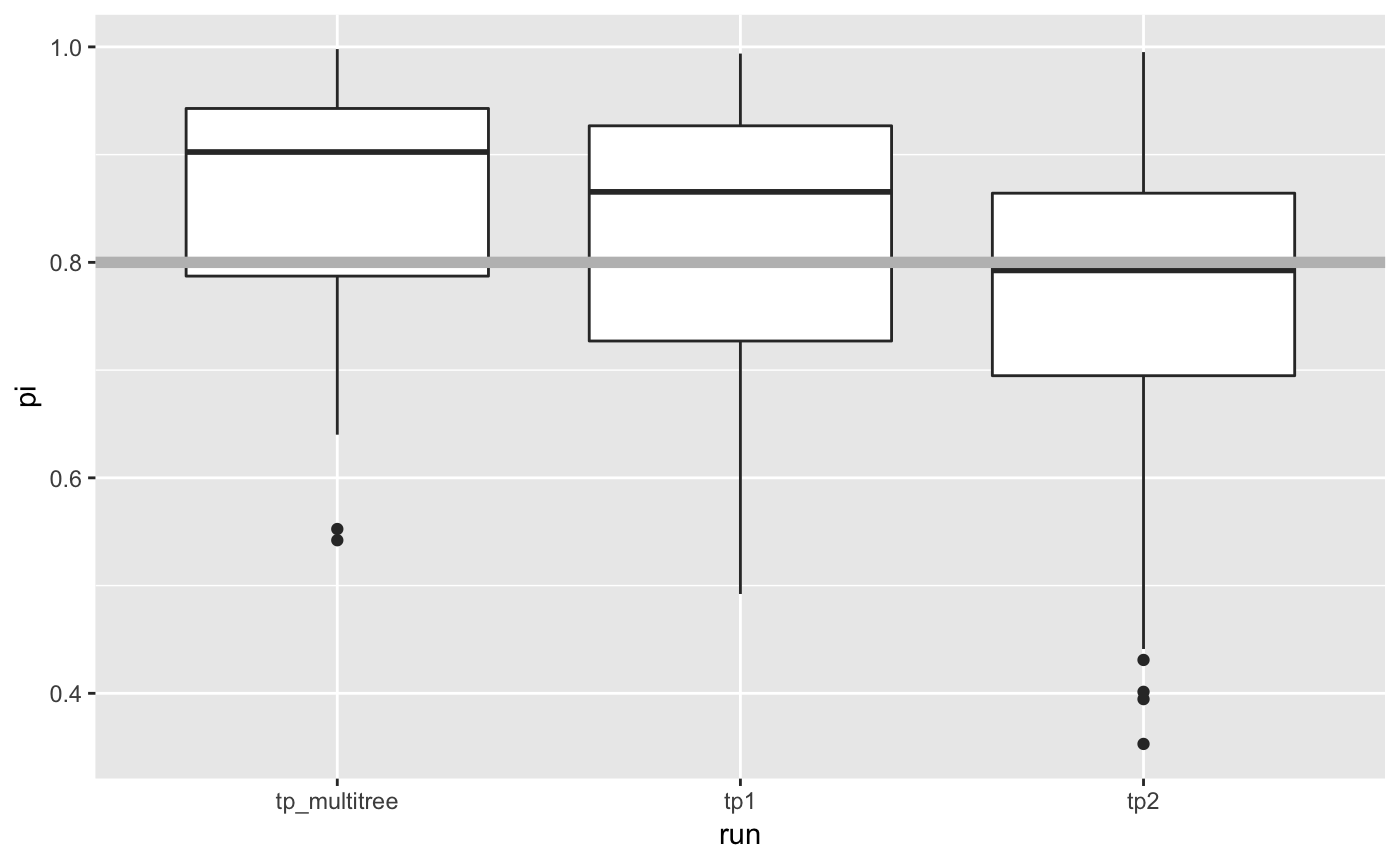
\includegraphics[width=4in,height=4in]{figure/unnamed-chunk-5-1} 

}



\end{knitrout}

The phylogenetic tree can be extracted and converted into a phylo object from the ape package:

\begin{knitrout}
\definecolor{shadecolor}{rgb}{0.969, 0.969, 0.969}\color{fgcolor}\begin{kframe}
\begin{alltt}
\hlkwd{library}\hlstd{(ape)}
\hlstd{ptree}\hlkwb{<-}\hlkwd{ptreeFromFullTree}\hlstd{(simu)}
\hlstd{p}\hlkwb{<-}\hlkwd{phyloFromPtree}\hlstd{(ptree)}
\hlkwd{plot}\hlstd{(p)}
\end{alltt}
\end{kframe}

{\centering 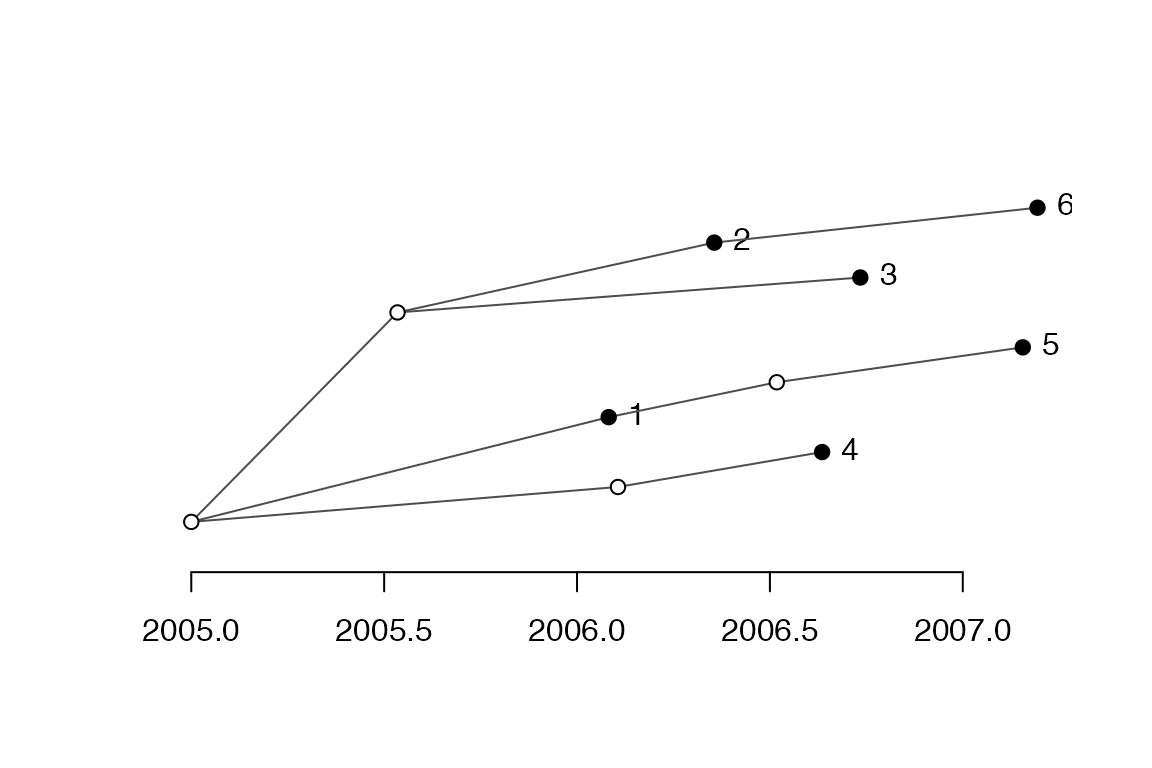
\includegraphics[width=4in,height=4in]{figure/unnamed-chunk-6-1} 

}



\end{knitrout}

\section{Inference of transmission tree given a phylogeny}

A phylo object can be turned  into a phylogenetic tree and complemented with a wild guess at the transmission tree in order to provide the starting point of the MCMC procedure:

\begin{knitrout}
\definecolor{shadecolor}{rgb}{0.969, 0.969, 0.969}\color{fgcolor}\begin{kframe}
\begin{alltt}
\hlstd{ptree}\hlkwb{<-}\hlkwd{ptreeFromPhylo}\hlstd{(p,}\hlkwc{dateLastSample}\hlstd{=}\hlkwd{max}\hlstd{(simu[,}\hlnum{1}\hlstd{]))}
\hlstd{full}\hlkwb{<-}\hlkwd{makeFullTreeFromPTree}\hlstd{(ptree)}
\hlkwd{plotBothTree}\hlstd{(full)}
\end{alltt}
\end{kframe}

{\centering 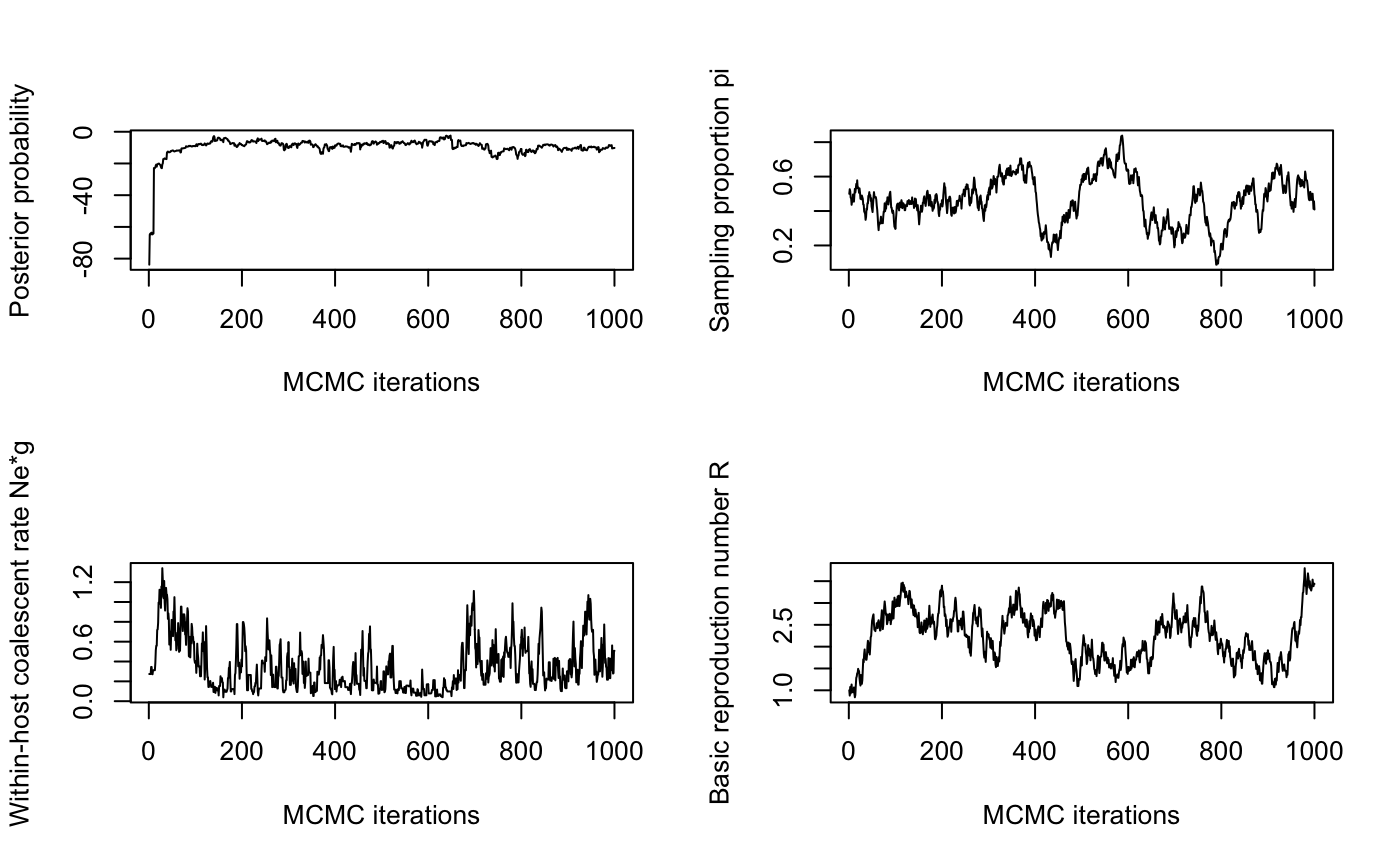
\includegraphics[width=4in,height=4in]{figure/unnamed-chunk-7-1} 

}



\end{knitrout}

The MCMC procedure to infer the transmission tree given the phylogenetic tree can be run as follows:

\begin{knitrout}
\definecolor{shadecolor}{rgb}{0.969, 0.969, 0.969}\color{fgcolor}\begin{kframe}
\begin{alltt}
\hlstd{record}\hlkwb{<-}\hlkwd{inferTTree}\hlstd{(ptree,}\hlkwc{mcmcIterations}\hlstd{=}\hlnum{1000}\hlstd{)}
\end{alltt}
\end{kframe}
\end{knitrout}

This returns a record of all MCMC iterations. This is what the transmission tree looks like at the end of the MCMC:

\begin{knitrout}
\definecolor{shadecolor}{rgb}{0.969, 0.969, 0.969}\color{fgcolor}\begin{kframe}
\begin{alltt}
\hlstd{lastIteration}\hlkwb{<-}\hlstd{record[[}\hlkwd{length}\hlstd{(record)]]}
\hlkwd{plotBothTree}\hlstd{(lastIteration}\hlopt{$}\hlstd{tree)}
\end{alltt}
\end{kframe}

{\centering 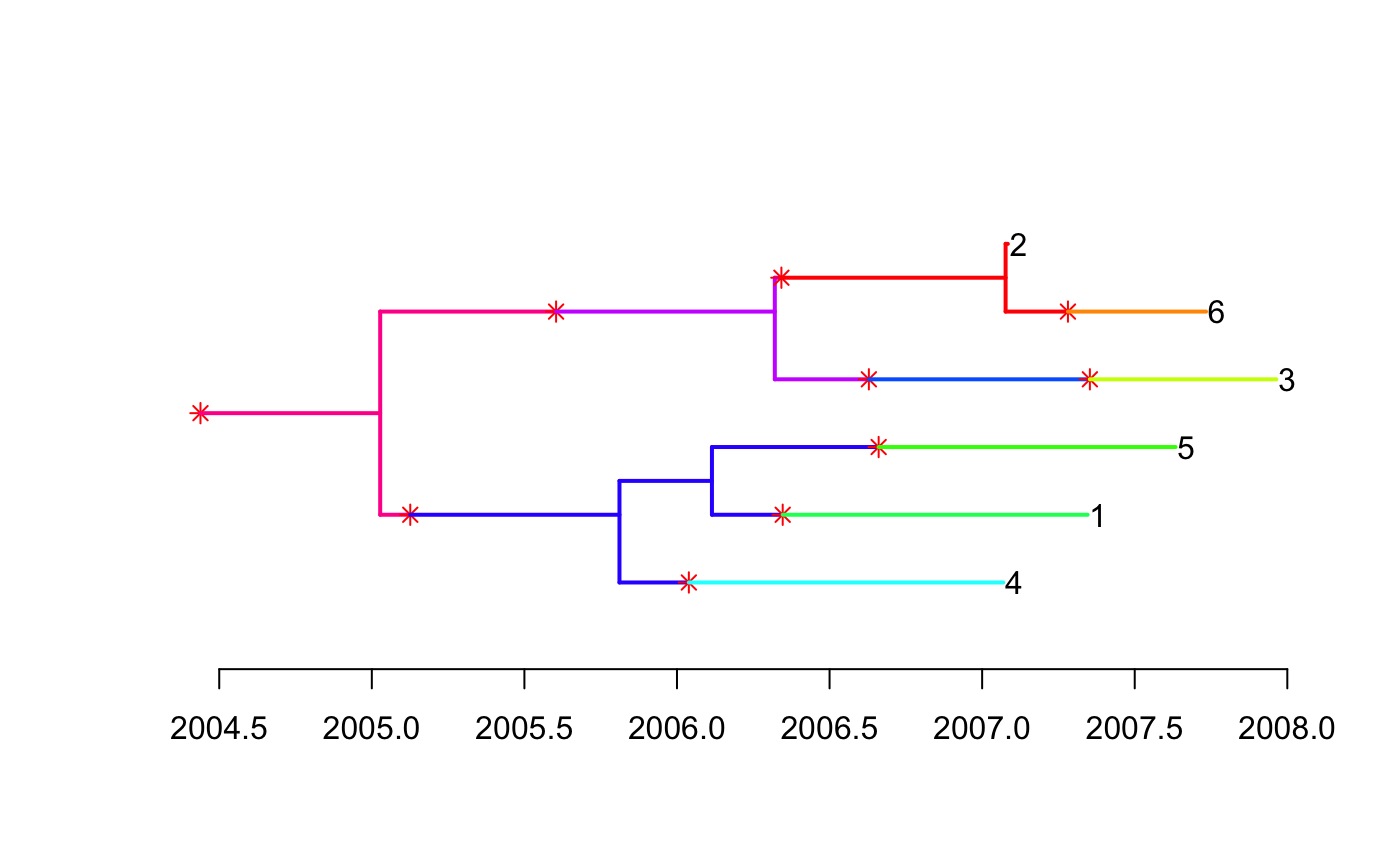
\includegraphics[width=4in,height=4in]{figure/unnamed-chunk-9-1} 

}



\end{knitrout}

Traces of the MCMC:

\begin{knitrout}
\definecolor{shadecolor}{rgb}{0.969, 0.969, 0.969}\color{fgcolor}

{\centering 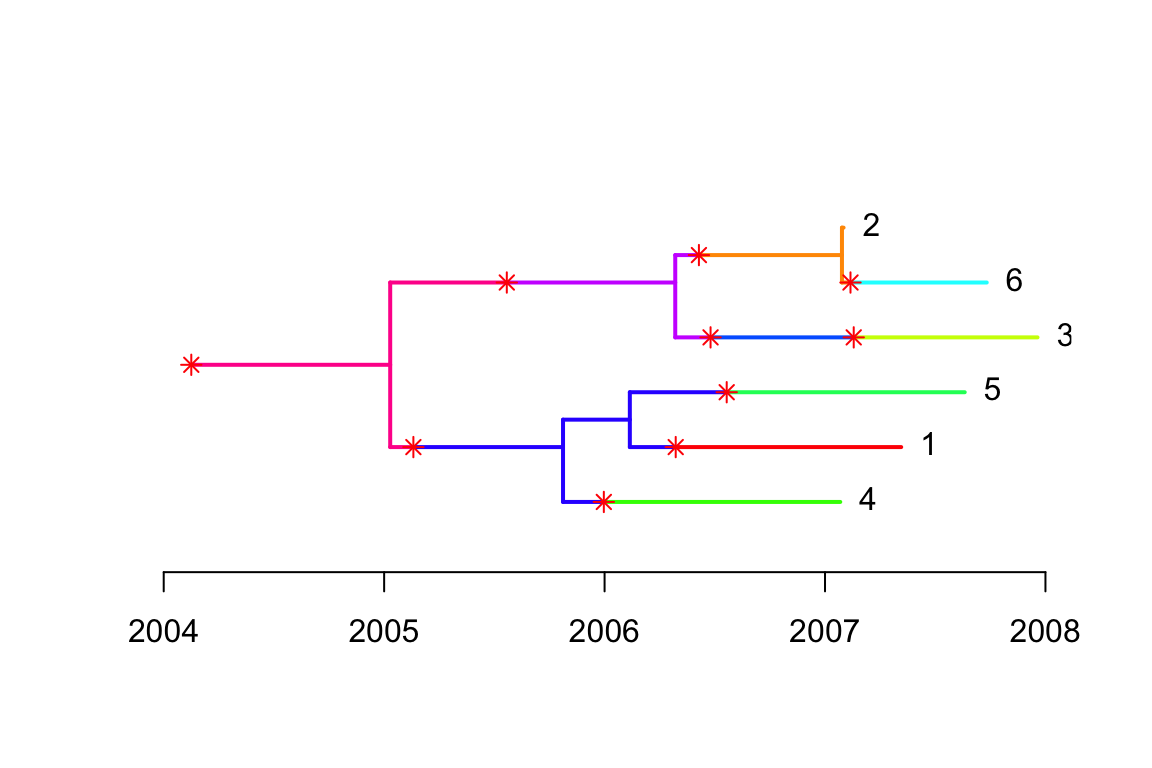
\includegraphics[width=4in,height=4in]{figure/unnamed-chunk-10-1} 

}



\end{knitrout}

\end{document}
